\laborator{Проектный и поверочный расчет абсорбера}

\goal для заданной модели структуры потока по жидкой и газовой фазам составить математическую модель процессов физической и химической абсорбции; на основе полученных моделей провести моделирование данных процессов в абсорбере, заполненном насадочными контактными элементами; результаты представить графически (в виде кривых равновесия и изменения концентрации абсорбтива по высоте аппарата в газовой и жидкой фазах).

\subsubsection{Теория}
Абсорбцией называется избирательное поглощение компонентов паровых или газовых смесей жидким поглотителем. Различают физическую абсорбцию и хемосорбцию.

При физической абсорбции растворение газа не сопровождается химической реакцией (или, по крайней мере, эта реакция не оказывает заметного влияния на процесс). В данном случае парциальное давление распределяемого компонента в газовой фазе превышает равновесное и его поглощение происходит до тех пор, пока его парциальное давление в газовой фазе будет выше равновесного давления над раствором. Физическая абсорбция обычно обратима. На этом свойстве абсорбционных процессов основано выделение поглощенного газа из раствора --- десорбция.

При хемосорбции абсорбируемый компонент связывается в жидкой фазе в виде химического соединения. Химическая реакция может быть как обратимой, так и необратимой. При необратимой реакции равновесное давление компонента над раствором становится близким к нулю и соответственно возможно его более полное извлечение из газовой фазы. При обратимой реакции давление компонента над раствором будет больше, чем при необратимой реакции, но меньше, чем в случае процесса физической абсорбции.

Участвующие в процессе абсорбции рабочие агенты имеют следующие названия:
абсорбтив --- распределяемый компонент газовой фазы, переходящий в жидкую;
инерт (инертный газ) -- компонент газовой смеси, не переходящий границу раздела фаз;
абсорбент --- жидкий поглотитель.

При абсорбционных процессах массообмен происходит на поверхности соприкосновения фаз. Поэтому абсорбционные аппараты должны иметь развитую поверхность соприкосновения между газом и жидкостью. Абсорбционные аппараты подразделяют на две групп:
\begin{itemize}
\item аппараты с непрерывным контактом фаз;
\item аппараты со ступенчатым контактом фаз.
\end{itemize}

В промышленности наибольшее распространение получили насадочные абсорберы, относящиеся к первой группе. В насадочных аппаратах жидкость стекает по поверхности загруженной в абсорбер насадки из тел различной формы (кольца, кусковой материал и т.д.). Для данных аппаратов поверхность контакта определяется геометрической поверхностью элементов насадки и гидродинамическим режимом работы колонны.
\begin{wrapfigure}{H}{0.5\textwidth}
	\begin{center}
		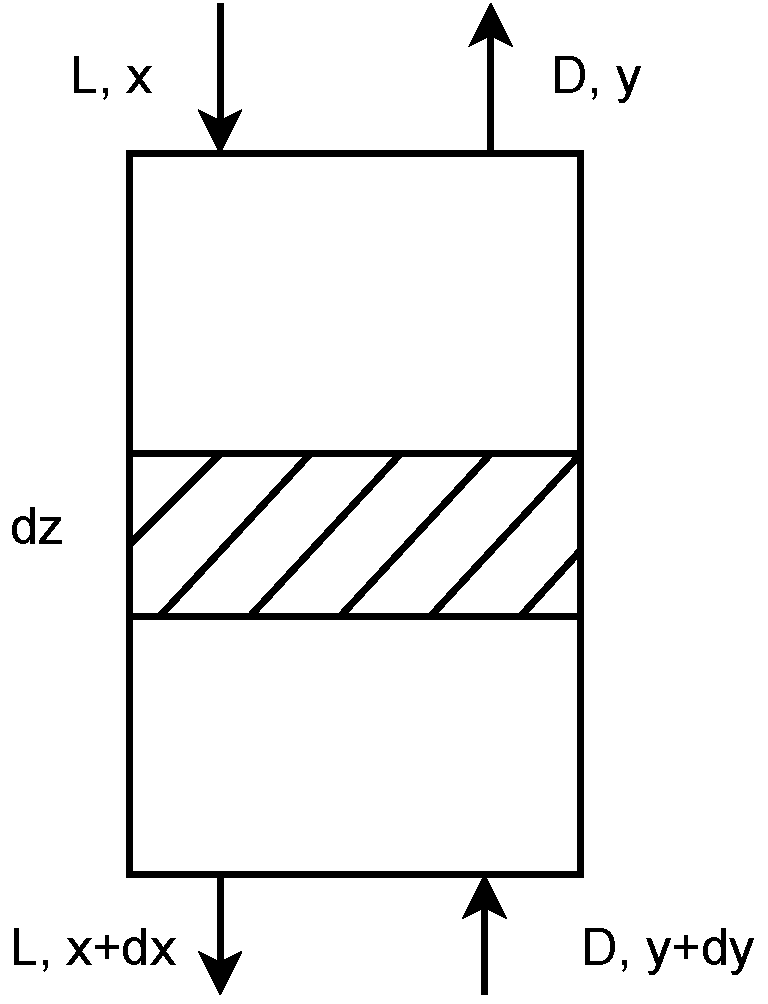
\includegraphics[width=0.48\textwidth]{flowscheme.pdf}
	\end{center}
	\caption{ Схема проведения процесса абсорбции (противоточная)} \label{fig:mass.sheme}
\end{wrapfigure}

В насадочной колонне контакт фаз осуществляется непрерывно. Данное обстоятельство приводит к необходимости использования для математического описания насадочных колонн дифференциальных уравнений, определяющих изменение концентрации распределяемого компонента в потоках по высоте колонны. Это соответственно позволяет определить изменение движущей силы процесса по высоте аппарата.

Математическое описание процесса физической абсорбции одного компонента в предположении, что движение потоков газа и жидкости описываются гидродинамическими моделями идеального вытеснения, будет состоять из системы двух дифференциальных уравнений, определяющих распределение его концентрации в потоках газа и жидкости. Для расчетов систему координат удобно расположить в верхней части аппарата (рисунок \ref{fig:mass.sheme}), так как в этом случае известны граничные условия: конечная концентрация абсорбтива в газе (степень извлечения задается в исходных данных); начальная концентрация абсорбтива в абсорбенте (принимается равной нулю или задается в исходных данных). В этом случае уравнения материального баланса по распределяемому компоненту для элементарного объема  запишутся следующим образом:
\begin{equation}
	L X - L(X +dX) + K_y a (Y-Y^*(X))Sdz=0, 
\end{equation}
\begin{equation}
	G(Y-dY)-K_y a (Y-Y^*(X))Sdz- GY=0,
\end{equation}
где $G$, $L$ --- массовый расход инертного носителя и абсорбента соответственно; $Y$, $X$ --- относительные массовые концентрации абсорбтива в газовой [кг А/кг В] и жидкой фазах [кг А/кг C] соответственно (А --- абсорбтив; В --- инертный газовый носитель; С --- абсорбент); $Y^*$ --- равновесная концентрация абсорбтива в газовой фазе [кг А/кг В]; $S$ --- площадь поперечного сечения аппарата; $а$ --- удельная активная поверхность контакта фаз; $K_y$ --- поверхностный коэффициент массопередачи. Таким образом, математическая модель процесса физической абсорбции одного компонента запишется в следующем виде:
\begin{equation}
\left\lbrace 
\begin{gathered} 
\dfrac{dX}{dz}=\dfrac{S}{L} K_Y a (Y-Y^*(X)),
\\
\dfrac{dY}{dz}=\dfrac{S}{G} K_Y a (Y-Y^*(X)).
\end{gathered} 
\right.
\end{equation}

В случае процесса хемосорбции химическая реакция, сопровождающая процесс абсорбции, может оказывать существенное влияние на кинетику процесса. При этом скорость процесса абсорбции определяется не только интенсивностью массопереноса, но и скоростью протекания химической реакции. Если реакция идет в жидкой фазе, то часть газообразного компонента переходит в связанное состояние. При этом концентрация свободного (т.е. не связанного химически) компонента в жидкости снижается, что приводит к увеличению движущей силы процесса и соответственно к ускорению процесса абсорбции. В общем случае скорость хемосорбции зависит как от скорости реакции, так и от скорости массопереноса между фазами. В зависимости от того, какая скорость определяет общую скорость процесса переноса массы, различают следующие области процессов хемосорбции:
\begin{itemize}
	\item кинетическую – скорость химического взаимодействия меньше скорости массопереноса, и поэтому лимитирует скорость всего процесса;
	\item  диффузионную – лимитирующей является скорость диффузии компонентов в зоне реакции, зависит от гидродинамических условий в системе и физических свойств;
	\item смешанная (диффузионно-кинетическая) – скорости химической реакции и массопередачи соизмеримы.
\end{itemize}

При моделировании процесса хемосорбции химическую реакцию можно учесть путем введения источника массы, который будет определять скорость образования или исчезновения компонента в элементарном объеме жидкой фазы. Обычно учет химической реакции осуществляется путем введения в математическую модель кинетического уравнения, определяющего скорость реакции. Если рассматривать химическую реакцию, протекающую в процессе хемосорбции, как элементарную:
\begin{equation}
	n_A A + n_B B \rightarrow n_c C,
\end{equation}
где $n$ --- соответствующие химической реакции стехиометрические коэффициенты, то кинетическое уравнение будет выглядеть следующим образом:
\begin{equation}
	r=k X_A^{n_A} X_B^{n_B},
\end{equation}
где $Х$ --- концентрации соответствующих компонентов. В случае, если порядок реакции по каждому из компонентов равен единице ($n_A=n_B=1$),  кинетическое уравнение запишется в виде
\begin{equation}
r=k X_A X_B.
\end{equation}

Данный вид уравнения справедлив, если проводить реакцию при близких концентрациях обоих компонентов. В процессах хемосорбции химически активные поглотители применяют большей частью в виде растворов, состоящих из инертной жидкости (растворителя) и активной части, причем активная часть находится в избытке относительно поглощаемого компонента. При проведении одной и той же реакции, но в условиях большого избытка одного из реагентов, концентрация вещества, находящегося в избытке, практически не изменяется (т.е. можно считать $X_B=const$) и может быть включена в константу скорости. Кинетическое уравнение в этом случае принимает вид
\begin{equation}
r=k' X_A, \quad k'=k X_B.
\end{equation}

Уравнение материального баланса в случае хемосорбции соответственно можно записать в виде:
\begin{equation}
L X - L(X +dX) + K_y a (Y-Y^*(X))Sdz-k'X=0, 
\end{equation}
\begin{equation}
G(Y-dY)-K_y a (Y-Y^*(X))Sdz- GY=0,
\end{equation}

Отсюда математическая модель процесса хемособции одного компонента запишется следующим образом:
\begin{equation}
\left\lbrace 
\begin{gathered} 
\dfrac{dX}{dz}=\dfrac{S}{L} K_Y a (Y-Y^*(X))-k'X,
\\
\dfrac{dY}{dz}=\dfrac{S}{G} K_Y a (Y-Y^*(X)).
\end{gathered} 
\right.
\end{equation}

Что касается константы скорости химической реакции, то она зависит от температуры по уравнению Аррениуса:
\begin{equation}
	k=k_0 e^{\frac{-E_a}{RT}},
\end{equation}
где $k_0$ --- предэкспоненциальный множитель, $E_a$ --- энергия активации, $R$ --- универсальная газовая постоянная, $Т$ --- температура. 

Оценка эффективности работы абсорбера как аппарата для поглощения компонента газовой смеси оценивают с помощью ряда параметров. Основным из них является степень извлечения компонента. Достигаемая степень извлечения зависит от технологического режима и совершенства как самого процесса, так и его аппаратурного оформления. Степень извлечения можно выразить посредством коэффициента извлечения:
\begin{equation}
	\phi =\dfrac{Y_н - Y_к}{Y_н - Y^*(X_н)},
\end{equation}
представляющего собой отношение количества поглощенного компонента к количеству, которое было бы поглощено при наиболее полном извлечении. Другими словами, он показывает количество поглощенного компонента к теоретическому, достигаемому в условиях равновесия между уходящим из абсорбера газом и вводимым компонентом. При полном извлечении $Y_к=0$, $\phi=1$ (при $Х_н=0$), во всех остальных случаях $\phi<1$.
 
При моделировании процессов химической технологии в зависимости от имеющейся входной и выходной информации, поставленных целей все решаемые задачи можно разделить на поверочные, проектные или проектно-поверочные.

Для проектной задачи требуется определить основные размеры аппарата (в случае процессов разделения это число ступеней разделения, теплообменных процессов --- поверхность теплообмена и т.д.) и режимные параметры процесса. Входная информация содержит данные о величине и составе входящих в аппарат потоков, а также ряд требований к выходящим потокам. 

Для поверочной задачи требуется определить величину и состав выходящих из аппарата потоков при заданных входящих потоках, параметрах аппарата (геометрия, схема потоков и др.) и режимных параметрах процесса. Входная информация содержит основные размеры аппарата и параметры процесса, характеристики всех входящих потоков. Выходная информация --- это характеристики выходящих потоков.

Проектно-поверочный расчет объединяет в одном цикле проектный и поверочный расчеты. 

В качестве примера приведем этапы при расчете пленочного абсорбера \cite{pavlov}. Исходными данными для проектирования являются: начальная концентрация поглощаемого компонента в газовой фазе $y_н \% моль.$, начальная концентрация поглощаемого компонента в абсорбенте $x_н \% моль.$, коэффициент поглощения $\phi$, расход поглощаемого газа $G \frac{кг}{ч}$, температура проведения процесса $t ^\circ C$, давление в абсорбере $p бар$.
Расчет конечной концентрации поглощаемого компонента в газе из условия заданного значения коэффициента поглощения $\phi$:
\begin{equation}
	y_к = (1-\phi) y_н.
\end{equation}
Пересчет начальных и конечных концентраций в газовой и жидкой фазах в относительно массовые доли:
\begin{equation}
	Y= \dfrac{y}{1-y}
\end{equation}

По уравнению Генри рассчитывается коэффициент распределения:
\begin{equation}
	 m = \dfrac{y^*(x)}{x}=\dfrac{E}{p},
\end{equation} 
где $E$ --- коэффициент Генри, $p$ --- давление  абсорбере. Значение константы Генри определяется исходя из температуры процесса по литературным источникам.

Вычисление объемного расхода газовой фазы при условиях в абсорбере:
\begin{equation}
	\dot{V} = \dfrac{G} {\rho_y} = \dfrac{G T  p_0}{\rho_{y0} T_0 p },
\end{equation}
где индекс $0$ соответствует нормальным условиям ($T_0=273.15 К$, $p_0 = 1.013 \cdot 10^5 Па$) $\rho_y=\frac{M}{22.4}$ --- плотность газа при нормальных условиях, $M$ --- молярная масса смеси.

Теоретический минимальный расход жидкой фазы определяется по материальному балансу, при условии, что газовая и жидкая фазы снизу колонны находятся в равновесии:
\begin{equation}
	L_{min} = \dfrac{G (Y_н - Y_к) } {Y_н /m - X_н}.
\end{equation}
В реальном аппарате расход абсорбента принимают выше:
\begin{equation}
	L = L_{min} \psi
\end{equation}
где $\psi$ --- коэффициент избытка поглотителя.
Рассчитывается фиктивная скорость захлебывания $w_з$ решением уравнения:
\begin{equation}
	\lg\left( \dfrac{w_з^2 \sigma \rho_y \mu_x^0.16} {g V_св^3 \rho_x} \right) = A -1.75 \left( \dfrac{L}{G} \right)^{0.25} \left( \dfrac{\rho_y}{\rho_x} \right)^{0.125}   
\end{equation}
где, $\sigma$ --- удельная поверхность насадки, $V_св$ --- свободный объема насадки, $\mu$ --- динамический коэффициент вязкости, индексы $x$ и $y$ соответствуют жидкой и газовой фазе, $A$ --- параметр, зависящий от типа насадки.

Рабочую скорость принимают ниже скорости захлебывания $w = (0.75 \div 0.9)w_з $ и исходя их этого определяют требуемый диаметр аппарата:
\begin{equation}
	D = \sqrt{\dfrac{4\bar{V}}{\pi w }}
\end{equation}
По найденному значению, подбирают ближайшее значение стандартного диаметра и проводят пересчет фиктивной скорости для нового значения диаметра:
\begin{equation}
	w = \dfrac{4 \bar{V}}{\pi D^2}.
\end{equation}

Далее определяются критерии Рейнольса для газовой:
\begin{equation}
	Re_y = \dfrac{4 w \rho_y}{\sigma \mu_y},
\end{equation}
и для жидкой фаз:
\begin{equation}
	Re_x = \dfrac{4 L}{S \sigma \psi \mu_x}.
\end{equation}
Критерии Прандтля определяется по выражению:
\begin{equation}
	Pr_y = \dfrac{\mu_y}{\rho_y D_y}
\end{equation}
где $D_y$ --- коэффициент диффузии поглощаемого компонента в газе. Критерий Прадтля для жидкой фазы определяется так же, как для газовой.

Критериальные уравнения для газовой фазы справедливо при значениях $Re$ от 10 о 10000:
\begin{equation}
	Nu_y = 0.407 Re_y^{0.655} Pr_y^{0.33},
\end{equation}
для жидкой фазы:
\begin{equation}
Nu_x = 0.0021 Re_x^{0.75} Pr_y^{0.5},
\end{equation}
Коэффициент массоотдачи с стороны газовой фазы определяется выражением:
\begin{equation}
	\beta_y = \dfrac{Nu_y D_y} {D},
\end{equation}
для жидкой фазы по выражению
\begin{equation}
\beta_x = \dfrac{Nu_x D_x}{\delta_{пр}},
\end{equation}
где $\delta_{пр} = \left( \dfrac{\mu_x^2} {\rho_x^2 g} \right)^{1/3} $ --- приведенная толщина жидкой пленки.

Далее определяется величина коэффициента массопередачи:
\begin{equation}
 K_y = \dfrac{1}{\dfrac{1}{\beta_y} + \dfrac{m}{\beta_x}}
\end{equation}

\subsubsection*{Вопросы для самоконтроля}
\begin{enumerate}
	\item Процессы абсорбции и хемосорбции. Для решения каких практических задач применяют эти процессы?
	\item Что такое процесс десорбции?
	\item Как составляется материальный баланс процессов абсорбции и хемосорбции?
	\item Дайте определение процесса массопередачи и коэффициента, характеризующего его скорость.
	\item Движущая сила процесса абсорбции.
	\item Как провести оценку эффективности работы абсорбера?
\end{enumerate}

\subsubsection*{Пример задания}
